\section{Cele pracy}
	Narzędzie powstało głównie w celach dydaktycznych -- ma ona na celu ułatwienie wizualizacji i tym samym zrozumienie początkującemu programiście działania algorytmów utworzonych w językach bazujących na języku C poprzez bezpośrednie pokazanie schematu blokowego odnoszącego się do napisanego kodu. Dodatkowo jest to przydatne narzędzie umożliwiające tworzenie schematów blokowych w łatwy i szybki sposób, wymagający jedynie podstaw programowania do dowolnego zastosowania. Narzędzie powinno również umożliwiać użytkownikom łatwe udostępnianie schematów innym użytkownikom w formie, którą łatwo można poddać dalszej edycji.
	
\section{Przykłady istniejących rozwiązaniań dla rysowania schematów blokowych typu flowchart}
	\subsection{Edytor graficzny} 
	Użycie dowolnego edytora graficznego -- jest to najmniej wydajne rozwiązanie -- rysowanie diagramów w ten sposób jest czasochłonne oraz trudne do ewentualnej edycji. Również wymaga od użytkownika dobrej znajomości edytora. Jedyną zaletą na tle innych rozwiązań jest nieograniczenie wyniku końcowego do predefiniowanych form -- daje największą swobodę.
		
	\subsection{Narzędzie do ręcznego rysowania schematów} 			
	Narzędzie specjalnie przeznaczone do rysowania za pomocą ręcznego umieszczania pojedyńczych bloczków oraz ich opisywania i łączenia np. \href{https://www.lucidchart.com/pages/examples/flowchart_software}{lucidchart} -- dużo wydajniejsze niż w przypadku użycia edytora graficznego dzięki gotowym elementom, które użytkownik może umieszczać i edytować w dość dużym zakresie.
		
	\subsection{Konwerter kodu na schemat blokowy} 	
	\begin{itemize}
	\item
	Narzędzie posiadające swoją własną składnie, stworzoną specjalnie na potrzeby rysowania diagramów (m. in. blokowych typu flowchart). Składnia sama w sobie zwykle jest dość prosta, jednak kod wymagany do stworzenia schematu blokowego w żaden sposób nie reprezentuje algorytmu, który przedstawia, a w bardziej złożonych przypadkach jest on nieczytelny co znacznie utrudnia i spowalnia pracę użytkownika. Jednym z wielu przykładów takiego narzędzia jest \href{https://mermaid-js.github.io/mermaid/#/}{Mermaid} -- używany dalej w tym projekcie jako język pośredniczący pomiędzy wprowadzanym kodem C-podobnym, a samym rysowaniem schematów na stronie HTML.
	
	\item
	Konwerter pseudo-kodu programistycznego wprost do schematu blokowego (którego wariantem jest ten projekt). Na rynku dostępna jest komercyjna wersja takiego konwertera pod nazwą \href{https://code2flow.com}{code2flow}. Zaletą tych rozwiązań jest wielokrotnie wyższa wydajność rysowania schematu oraz bezpośrednie odniesienie go do napisanego kodu co daje lepszą gwarancje poprawności rozwiązania oraz najłatwiejszą edycję spośród wszystkich dostępnych metod. Na niekorzyść tej metody działa jedynie jej mała elastyczność -- użytkownik ma niewielki wpływ na końcowy wygląd schematu, jest to w dużej mierze wstępnie zdefiniowane przez twórców tego typu narzędzi.
	\end{itemize}
	
\begin{figure}[h]
    \centering
\begin{minipage}[b]{.33\textwidth}
    \centering
   %\begin{flalign} 
   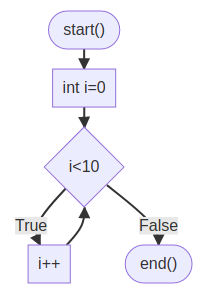
\includegraphics[width=.9\linewidth]{decyzja-while.png}
   %\end{flalign}   
\end{minipage}%
\hfill\vline\hfill
\hspace{0.02\linewidth}
\begin{minipage}[b]{0.3\textwidth}
    \centering 
%\begin{flalign}
\strut\vspace*{-\baselineskip}\newline\
C:
\begin{minted}{cpp}
  
start();
int_ i = 0;
while(i < 10){
  i++;
}
end();
  \end{minted}
%\end{flalign}
\end{minipage}%
\hfill\vline\hfill
\hspace{0.02\linewidth}
\begin{minipage}[b]{0.3\textwidth}
    \centering
    %\begin{flalign}
    \strut\vspace*{-\baselineskip}\newline\
    Mermaid:
  	\begin{minted}{python}
graph TD;
N1(["start()" ]);
N2["int i=0" ];
N5{"i<10" };
N6["i++" ];
N7(["end()" ]);
N1-->N2;
N2-->N5;
N5-->|True|N6;
N5-->|False|N7;
N6-->N5;
  	\end{minted}
   %\end{flalign}

    \end{minipage}
    \label{fig:prob3}
    \caption{Porównanie składni obu typów konwerterów, które generują ten sam schemat blokowy.}
\end{figure}
	

	
\section{Forma pracy}
	Praca ma charakter projektowy i polega na stworzeniu narzędzia, za pomocą którego będzie można w łatwy sposób narysować (wygenerować) schematy blokowe typu flowchart na podstawie elementów składniowych zaczerpniętych z języka C, takich jak:

\begin{itemize}
	\item {
		wywołanie funkcji lub przypisanie -- jako bloczek procesu
	}
	\item instrukcje warunkowe typu $if / else$ -- bloczek decyzyjny z dwiema gałęziami reprezentującymi wykonywanie kolejnych instrukcji w zależności od warunku podanego wewnątrz bloczka decyzyjnego,
	\item  instrukcja warunkowego wykonywania pętli $while$ -- jako bloczek decyzyjny, wraz z pętlą wskazującą na ten bloczek po zakończeniu instrukcji zawartych poniżej.
\end{itemize}

  Generator (podobnie jak kompilator języka C) obsługuje zagnieżdżenie w sobie powyższych instrukcji (tzn. można rozbudować drzewko decyzyjne umieszczając jedną instrukcję warunkową wewnątrz drugiej). Aplikacja jest w stanie zinterpretować jedynie wyżej wymienione instrukcje, które są wystarczające do stworzenia większości algorytmów w praktyce. Odstępstwami i jednocześnie brakami w porównaniu do języka C jest brak takich instrukcji jak: for, do-while oraz goto. Z punktu widzenia samego działania algorytmu, każdą pętle for oraz do-while można zastąpić najbardziej podstawową pętlą while -- w przypadku for: zadeklarowanie dodatkowych zmiennych przed pętlą oraz wywołanie dodatkowej instrukcji na końcu każdej iteracji pętli, natomiast w przypdaku do-while: zamiana warunku głównego pętli na wewnętrzne warunki wywołania instrukcji continue lub break. instrukcja goto została pominięta ponieważ również można ją w pełni zastąpić pętlami, używanie tej instrukcji uchodzi również za złą praktykę programistyczną.  Dodatkowo w związku z tym, że interfejsem aplikacji jest formularz HTML, wywołujący zapytania do serwera poprzez Rest API, po udostępnieniu aplikacji np. na platformie chmurowej, będzie można w łatwy sposób udostępniać utworzony schemat wraz z kodem na podstawie którego powstał za pomocą linku. Dodatkową funkcjonalnością jest również obsługa znaków Unicode, co umożliwia pisanie kodu z użyciem m.in. polskich znaków oraz zawijanie tekstu w bloczkach, zapobiegając nadmiernemu rozrostowi bloczków przy większej ilości tekstu.
  
\section{Wykorzystane narzędzia i technologie wraz z opisem}
	Wszystkie użyte technologie i narzędzia są open-source i do ich użytku (nawet komercyjnego) nie wymagają żadnych dodatkowych obligacji:

\begin{itemize}
	\item HTML5, CSS, Thymeleaf -- interfejsem aplikacji będzie prosty formularz w formie strony internetowej uzyskanej metodą szablonu HTML, komunikującej się z serwerem poprzez Rest API.	
	
	\item Mermaid -- narzędzie napisane w JavaScript umożliwiające rysowanie schematów na stronie HTML	za pomocą specjalnej składni, unikalnej dla tego narzędzia.
	
	\item Java 11 SE, Spring Boot framework -- część back-endowa aplikacji w którą m. in. wchodzą: obsługa zapytań Rest API, implementacja klas i zawartych w nich algorytmów interpretujących język C-podobny oraz zamieniających go na język wymagany przez narzędzie do rysowania schematów (Mermaid)
	
	\item Użyte narzędzia programistyczne: IntelliJ IDEA Community Edition, Visual Studio Code, system kontroli wersji Git.
		
		
\end{itemize}
	